\documentclass{beamer}
\usepackage[francais]{babel}
\usepackage[utf8]{inputenc}
\usepackage[T1]{fontenc}
\usepackage{multicol}

\usetheme{Berlin}

\usepackage{listings}
\usepackage{xcolor}

\definecolor{mygreen}{rgb}{0,0.6,0}
\definecolor{mygray}{rgb}{0.3,0.3,0.3}
\definecolor{mymauve}{rgb}{0.58,0,0.82}

\lstset{ %
  backgroundcolor=\color{white},   % cbackground color \usepackage{xcolor}
  basicstyle=\footnotesize,        % font size
  breakatwhitespace=false,         % autobreak only at whitespace
  breaklines=true,                 % sets automatic line breaking
  captionpos=b,                    % sets the caption-position to bottom
  commentstyle=\color{mygreen},    % comment style
  deletekeywords={...},            % delete keywords from the given language
  escapeinside={\%*}{*)},          % if you want to add LaTeX within your code
  extendedchars=true,              % lets you use non-ASCII characters; no UTF8
  frame=single,                    % adds a frame around the code
  keepspaces=true,                 % keeps spaces, to indent : columns=flexible
  keywordstyle=\color{blue},       % keyword style
  language=Octave,                 % the language of the code
  morekeywords={*,...},            % if you want to add more keywords to the set
  numbers=left,                    % where to put line number (none, left, right)
  numbersep=5pt,                   % how far the line-numbers are from the code
  numberstyle=\footnotesize\color{mygray}, % line number style
  rulecolor=\color{white},         % black for rules
  showspaces=false,                % show spaces, overrides 'showstringspaces'
  showstringspaces=false,          % underline spaces within strings only
  showtabs=false,                  % show tabs 
  stepnumber=1,                    % the step between two line-numbers.
  stringstyle=\color{mymauve},     % string literal style
  tabsize=2,                       % sets default tabsize to 2 spaces
  title=\lstname                   % filename \lstinputlisting; try caption
}

\lstdefinestyle{customc}{
  belowcaptionskip=1\baselineskip,
  breaklines=true,
  frame=L,
  xleftmargin=\parindent,
  language=C,
  showstringspaces=false,
  basicstyle=\normalsize\ttfamily,
  keywordstyle=\bfseries \color{green!40!black},
  commentstyle=\itshape \color{purple!40!black}, %itshape
  identifierstyle=\color{blue},
  stringstyle=\color{orange},
}
\lstset{escapechar=@,style=customc}



\defbeamertemplate*{headline}{}
{
  \begin{beamercolorbox}[ht=2.25ex,dp=3ex,center]{section in head/foot}
    \insertnavigation{\paperwidth}
  \end{beamercolorbox}
}
 
\defbeamertemplate*{footline}{infolines}
{l
  \leavevmode%
  \hbox{%
  \begin{beamercolorbox}[wd=.5\paperwidth,ht=2.25ex,dp=1ex,center]{title in head/foot}
    \usebeamerfont{title in head/foot}\insertshorttitle
  \end{beamercolorbox}%
  \begin{beamercolorbox}[wd=.5\paperwidth,ht=2.25ex,dp=1ex,right]{date in head/foot}
    \usebeamerfont{date in head/foot}%\insertshortdate{}\hspace*{2em}
    ENSEIRB-MATMECA\hspace*{4em}
    \insertframenumber{} / \inserttotalframenumber\hspace*{4em}
  \end{beamercolorbox}}
  \vskip0pt%
}

\title{Projet Olimex}
\author{Mathias Brulatout \and Arnaud Duforat \and Louis Lévêque \\ Kamal Mallouky \and Nicolas Sarlin}
\institute{Responsable Pédagogique : \\ Aymeric Vincent}
\titlegraphic{\includegraphics[scale=0.16]{enseirb.png}}
\date{\today}
\makeatletter
\newenvironment{withoutheadline}{
  \setbeamertemplate{headline}[default]
  \setbeamertemplate{footline}[default]
  \def\beamer@entrycode{\vspace*{-\headheight}}
}{}
\makeatother
\begin{document}
\begin{withoutheadline}
  \begin{frame}
    \titlepage
  \end{frame}
\end{withoutheadline}
\addtocounter{framenumber}{-1}


\AtBeginSection[]
{
  \begin{frame}
    \frametitle{Sommaire}
    \tableofcontents[currentsection]
  \end{frame}
}
\begin{frame}
  \frametitle{Sommaire}
  \tableofcontents
\end{frame}


\section{Existant}
\subsection{}
\begin{frame}
  \frametitle{OLinuXino A20}
  \begin{itemize}
  \item Micro-ordinateur
  \item System on Chip (SoC)
  \item Système Android installé
  \item divers composants
    \begin{itemize}
      \item USB/HDMI/Eth...
      \item 8 UARTs
      \item 3GPIOs = 160pins
    \end{itemize}
  \end{itemize}
\end{frame}


\begin{frame}
  \frametitle{Uboot}
  \begin{itemize}
  \item Chargeur de démarrage open-source
  \item Plusieurs architectures
  \item Initialise les périphériques
  \item Charge l'OS
  \end{itemize}
\end{frame}

\section{Architecture}
\subsection{ }

\begin{frame}
\frametitle{Architecture}
\begin{itemize}
\item Modulaire
    \begin{itemize}
	\item Communication série
	\item Interface console
	\item Commandes
	\item Gestion périphériques
    \end{itemize}
\item Extensible
    \begin{itemize}
	\item Possibilité d'ajouter de nouvelles commandes
    \end{itemize}
\end{itemize}
\end{frame}

\begin{frame}
\frametitle{Architecture}
\begin{itemize}
\item baremetal\_os.c
\item uart.c
\item console.c
\item gpio.c
\item led.c
\item memory.c
\item command.c
\end{itemize}
\end{frame}

\begin{frame}[fragile]
\frametitle{Structure cmd}
\begin{lstlisting}
struct cmd {
  char * name;
  char * desc;
  int nb_arg;
  struct arg args[MAX_ARGS];
  //Function to call
  int (*func)(const char * arg, int nb_args);
};
\end{lstlisting}
\end{frame}

\section{UART}
\subsection{}
\begin{frame}
  \frametitle{Principe}
  Différents registres :
  \begin{itemize}
    \item Contrôle
    \item Status
    \item Data
  \end{itemize}~\\
  \textsf{getc} \& \textsf{putc} \\~\\
  Emulation d'un terminal
\end{frame}

\begin{frame}
\frametitle{Commandes possibles}
  \textsf{led} \\
  \textsf{gpio pin\_number} \\
  \textsf{reg} \\
    \begin{itemize}
    \item Stack Pointer
    \item Link Register
    \item Proc Counter
    \end{itemize}
\end{frame}

\section{GPIO}
\subsection{ }

\begin{frame}
\frametitle{ }
\end{frame}

\section{Memory Management}
\subsection{ }
\begin{frame}
  \frametitle{Detection de la mémoire}
  \begin{itemize}
  \item Manual Probing
  \item Doc Reading
  \end{itemize}
\end{frame}

\begin{frame}[fragile]
  \frametitle{Affichage de l'état des registres}
\begin{lstlisting}  
unsigned int spReg, lrReg, pcReg;    
asm volatile ("mov %0, sp" :"=r" (spReg));   
asm volatile ("mov %0, lr" :"=r" (lrReg));
asm volatile ("mov %0, pc" :"=r" (pcReg));
\end{lstlisting}
\end{frame}

\begin{frame}
  \frametitle{Gestionnaire de mémoire}
  \begin{itemize}
  \item Taille du bloc écrite au début
  \item Pointeur vers la fin de la zone allouée
  \item Liste chainée des blocs libres avant ce pointeur
  \end{itemize}
\end{frame}

\begin{frame}
  \frametitle{Structure d'un bloc}
  \begin{itemize}
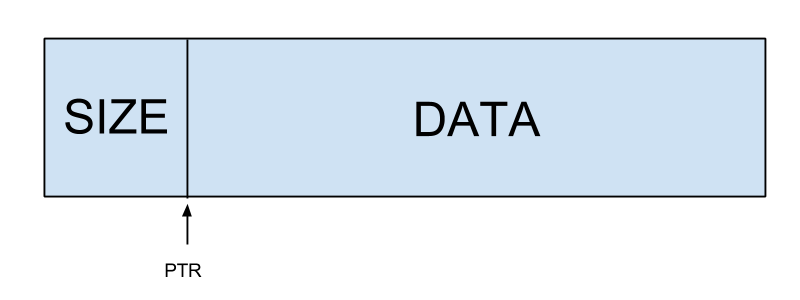
\includegraphics[width=8cm]{memblock.png}
  \end{itemize}
\end{frame}

\let\origaddtocontents=\addtocontents
\def\dontaddtocontents#1#2{}
\let\addtocontents=\dontaddtocontents
\section*{Conclusion}
\let\addtocontents=\origaddtocontents

\begin{frame}
  \frametitle{Conclusion}
  Régression U-boot \\~\\
  Utilisation des UARTs et GPIOs réussie \\~\\
  malloc/free implémentés \\~\\
\end{frame}

\end{document}
